\section{Experiment}\label{sec:experiment}
\autoref{fig:eva} shows the \replaced[id=kg]{FPS}{frame per second (FPS)} over datasets with varied sizes of \name and other \replaced[id=kg]{five}{5} tools\footnote{https://github.com/ZJUVAG/NetV.js/tree/benchmarks/benchmarks}, namely,  % We recorded the frame per second (FPS) experiment\footnote{https://github.com/ZJUVAG/NetV.js/tree/benchmarks/benchmarks} to test the rendering performance of \name with other popular tools and libraries which are supports graph rendering, including 
D3-SVG, D3-Canvas, Cytoscape.js, Sigma.js, and Stardust.js. In particular, \name, Sigma.js, and Stardust.js use WebGL. To simulate real-world graph data, we set the graph density as 20, which means the ratio of the number of edges to the number of nodes is 1 to 20. 
% The display refresh rate is 144Hz; the GPU is GTX 1060 with 6G.
Experiments are performed on a PC equipped with a GPU (NIVIDIA GTX 1060, 6G) and a monitor with a refresh\deleted[id=kg]{ing} rate of 144 HZ.

Stardust.js, and D3-Canvas can render up to 100 thousand elements. \added[id=kg]{Meanwhile, }\name can render more than 1 million elements with FPS greater than 1.

\begin{figure}[htbp]
    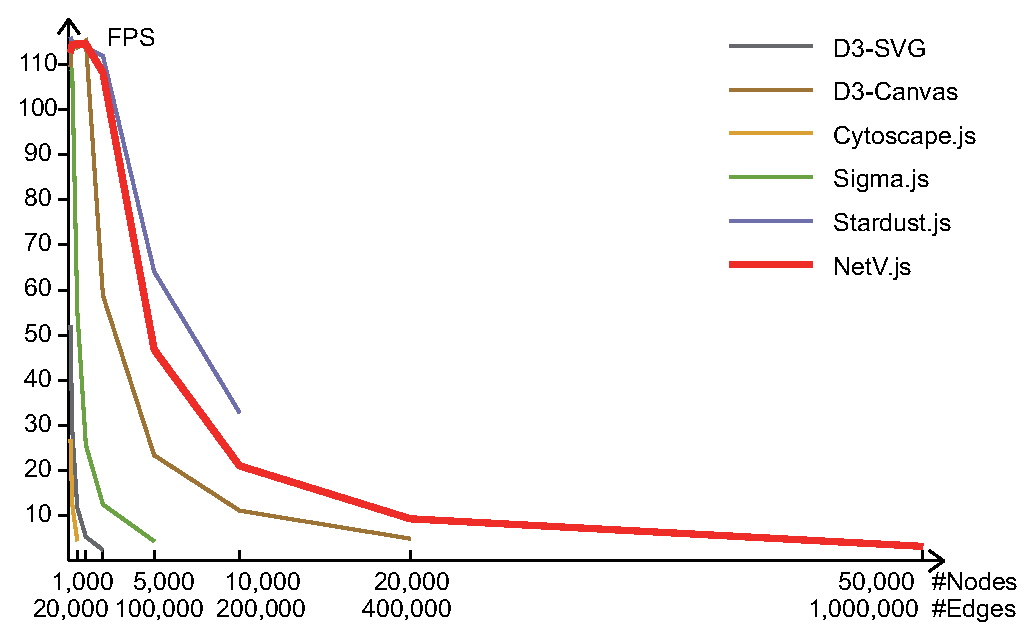
\includegraphics[width=\linewidth]{fig/eva.eps}
    \caption{
        Performance comparison among \replaced[id=kg]{six}{6} toolkits.
    }
    \label{fig:eva}
\end{figure}
